\documentclass{article}

\usepackage[preprint]{neurips_2020}
% \usepackage[final]{neurips_2020}
% \usepackage[nonatbib]{neurips_2020}

\usepackage[utf8]{inputenc} % allow utf-8 input
\usepackage[T1]{fontenc}    % use 8-bit T1 fonts
\usepackage{hyperref}       % hyperlinks
\usepackage{url}            % simple URL typesetting
\usepackage{booktabs}       % professional-quality tables
\usepackage{amsfonts}       % blackboard math symbols
\usepackage{nicefrac}       % compact symbols for 1/2, etc.
\usepackage{microtype}      % microtypography
\usepackage{graphicx}
\usepackage{subcaption}
\usepackage{float}

\title{Vector Quantized Variational Autoencoders \\on Novel Datasets}

\author{
  Shivanshu Gupta
  \And
  Kolby Nottingham
  \And
  Preethi Seshadri
}

\begin{document}

\maketitle

\begin{abstract}
    We explore using the Vector Quantized Variational Autoencoder (VQ-VAE) to generate discrete representations for the Kaokore dataset, which contains images of facial expressions from traditional Japanese illustrations (\url{https://github.com/rois-codh/kaokore}).
    The framework VQ-VAE is built on, Variational Autoencoders (VAE), learn continuous latent representations.
    While continuous representations are flexible, many real world attributes are better defined discretely, and some current state-of-the art model architectures, like transformers, only work with discrete data. Additionally, VAEs have been shown to exhibit posterior collapse, which means that latent codes are ignored. 
    In this project, we experiment with VQ-VAEs on a novel dataset and design experiments to test the advantages and disadvantages of multiple VQ-VAE variations.
    %Since the VQ-VAE paper uses CIFAR10 and 128x128 ImageNet images, there might be additional experimentation and training required to achieve good performance on the Kaokore dataset.
    % VQ-VAEs have been paired with the transformer architecture which, while scalable, can require a lot of compute, so we will experiment with making the method more compute efficient.  % Not sure what to put in this sentence??? Maybe something generic for now.
    Our results indicate that while the original VQ-VAE algorithm learns faster than some of its successors, it does not achieve the same level of performance. 
\end{abstract}

\section{Introduction}

Generative machine learning models learn a distribution $p(x,y)$ for data instances $x$ and labels $y$. Compared to discriminative machine learning models that learn $p(y|x)$, generative models can be more difficult to learn but come with added benefits. One use case for generative machine learning models is mapping data instances to a latent space. Once mapped to a latent space, latent variables can be used as a compressed representation of a data instances or to sample and generate new data instances.

One generative machine learning model that learns latent variable representations of data is the variational autoencoder (VAE). VAEs learn a latent variable representation of each datapoint with an encoder module. Simultanously, a decoder module learns to reconstruct the original image from the latent variables.

Traditional VAEs learn a latent space that is associated with a probablility distribution of continuous variables. Vector quantized variational autoencoders (VQ-VAE) learn discrete latent variables instead. Discrete variables are cometimes advantageous because real world data can often be summarized by categorical features. 

In this work, we compare two variations of VQ-VAEs. The second variation (VQ-VAE2) was released as a follow up to VQ-VAEs and introduces a hierarchical structure for the model. We go into further detail comparing the algorithms in section \ref{methods}. We implement each of these methods and run experiemnts with each on the Kaokore dataset. To the best of our knowledge, this is the first time VAEs have been used to learn a latent space for this dataset.

\section{Methods} \label{methods}
In this section, we will describe the various models used in this paper: VAE, VQ-VAE, and VQ-VAE2. While the continuous latent representation of VAEs offers benefits such as latent interpolation, having discrete latent representations can be a more natural fit for certain modalities. Additionally, it has been shown that VAEs can suffer from posterior collapse, a phenomenon in which the learned latent space becomes uninformative. VQ-VAEs have been formulated to address these concerns, while still offering similar performance to VAEs. 

\subsection{VAE}
Similar to vanilla autoencoders, variational autoencoders include an encoder which yields a lower dimensional latent representation and a decoder which reconstructs the input. However, VAEs compute an additional loss term that computes the Kullback-Leibler (KL) divergence between the encoder’s distribution \(q_{\theta}(z|x)\) and \(p(z)\), where \(p(z)\) is typically specified as a normal distribution with zero mean and unit variance. This term serves as a regularizer that keeps similar inputs’ latent representations close together.

From a generative modeling perspective, imagine data point \textit{i} is sampled by 1) drawing latent variable \(z_{i}\) and 2) drawing datapoint \(x_{i}\) based on \(z_{i}\). Therefore, we would like to infer a good latent representation \textit{z} given input \textit{x}. This is given by the posterior:

\begin{equation}
    p(z|x) = \frac{p(x|z)p(z)}{p(x)}
\end{equation}

However, computing the denominator \(p(x)\) requires marginalizing over latents \textit{z} and is often computationally intractable. Instead, variational inference allows us to approximate \textit{p(z|x)} through another distribution \textit{q(z|x)}, which is referred to as the approximate posterior. In other words, we would like to optimize the divergence between the approximate and original posteriors:

\begin{equation}
    \min{KL(q(z|x) \| p(z|x))} 
\end{equation}

The expression above cannot be optimized directly, since it requires computing \textit{p(x)}. While we do not go through the derivation here, minimizing the KL divergence between \textit{q(z|x)} and \textit{p(z|x)} is equivalent to maximizing the evidence lower bound (ELBO), which is computationally tractable. 

\begin{equation}
ELBO = E_{q_{\theta}(z|x)} \log{p_{\phi}(x|z)} - KL(q_{\theta}(z|x)||p(z))
\end{equation}

In practice, VAEs are modeled using neural networks; the approximate posterior is computed from the inference network (encoder) with parameters \(\theta\) and the likelihood is computed from the generative network (decoder) network with parameters \(\phi\). 
\subsection{VQ-VAE}
In order to learn discrete latent representations, the posterior and prior distributions are categorical instead of gaussian, and samples from these distributions are drawn by indexing an embedding table. The latent embedding space is \(e \in R^{K \times D}\), where \textit{K} is the size of the discrete latent space (i.e., a \textit{K}-way categorical) and \textit{D} is the dimensionality of each latent embedding vector \(e_{i}\).The discrete latent variables \textit{z} are calculated by a nearest neighbor look-up using the embedding table in a process referred to as Vector Quantization (VQ). Therefore, the forward computation pipeline can be viewed as a standard autoencoder with a non-linearity that maps the latents to one of \textit{K} embedding vectors. Since performing a nearest neighbors lookup is non-differentiable, straight-through gradient estimation is used so that the gradient passed back is the same before and after quantization. 

The loss function consists of three terms: 
\begin{enumerate}
\item Reconstruction loss: Encourages original and reconstructed images to be similar
\item Codebook loss: Encourages the embedding vectors \textit{e} to be close to the encoder output 
\item Commitment loss: Encourages the encoder output to be close to the embedding vectors \textit{e} 
\end{enumerate}

\begin{equation}
L = \log{p(x|z_q(x))} + {\|\textrm{sg}[z_e(x)]-e\|}_2 + \beta{\|z_e(x)-\textrm{sg}[e]\|}_2
\end{equation}


The decoder optimizes the first term only, the encoder optimizes the first and last terms, and the embeddings are optimized by the middle term. 

\subsection{VQ-VAE2}

VQ-VAE2 builds on VQ-VAE by using a hierarchical VQ-VAE model to encode images onto a discrete latent space, followed by learning a powerful PixelCNN prior. In this hierarchical architecture, the top-level latent code models global information and the bottom-level latent code, conditioned on the top-level latent, is responsible for representing local details. As a result the learned prior is also hierarchical; the top-level PixelCNN prior is conditioned on the class label, and the bottom level PixelCNN is conditioned on the class label as well as the top-level latent code. The authors show that the VQ-VAE2 framework produces samples that rival perceptual quality of GANs, while not suffering from lack of diversity. 

\section{Experiments}

In a series of experiments, we compare traditional VAEs to VQ-VAEs. We first...

\subsection{Kaokore Dataset}

The Kaokore dataset consists of facial expressions extracted from pre-modern Japanese artwork. The dataset focuses on cropped face images extracted from Japanese artwork from the Late Muromachi Period (16th century) to the Early Edo Period (17th century) to facilitate research on art history and artistic style. The most recent version contains 8848 colored images, and each image is annotated with gender (male, female) and social status (noble, warrior, incarnation, commoner) labels. The paper associated with the dataset looks at classification as well as generative modeling, such as neural painting and style transfer models. 

\subsection{Results}

\begin{table}[H]
    \centering
    \begin{tabular}{c c c}
        & Commitment Loss & Reconstruction Loss \\
        \hline
        VQ-VAE & 0.0793 (0.0027) & 0.0056 (0.0001) \\
        VQ-VAE2 & 0.0025 (0.0035) & 0.0005 (0.0008)
    \end{tabular}
    \caption{Commitment loss and reconstruction loss on the Kaokore testset for both algorithms.}
\end{table}

\begin{figure}[H]
    \centering
    \begin{subfigure}{.49\linewidth}
        \centering
        \includegraphics[width=\linewidth]{commit.png}
        \caption{Commitment loss over 100 epochs.}
    \end{subfigure}
    \begin{subfigure}{.49\linewidth}
        \centering
        \includegraphics[width=\linewidth]{recon.png}
        \caption{Reconstruction loss over 100 epochs.}
    \end{subfigure}
\end{figure}

\begin{figure}
    \centering
    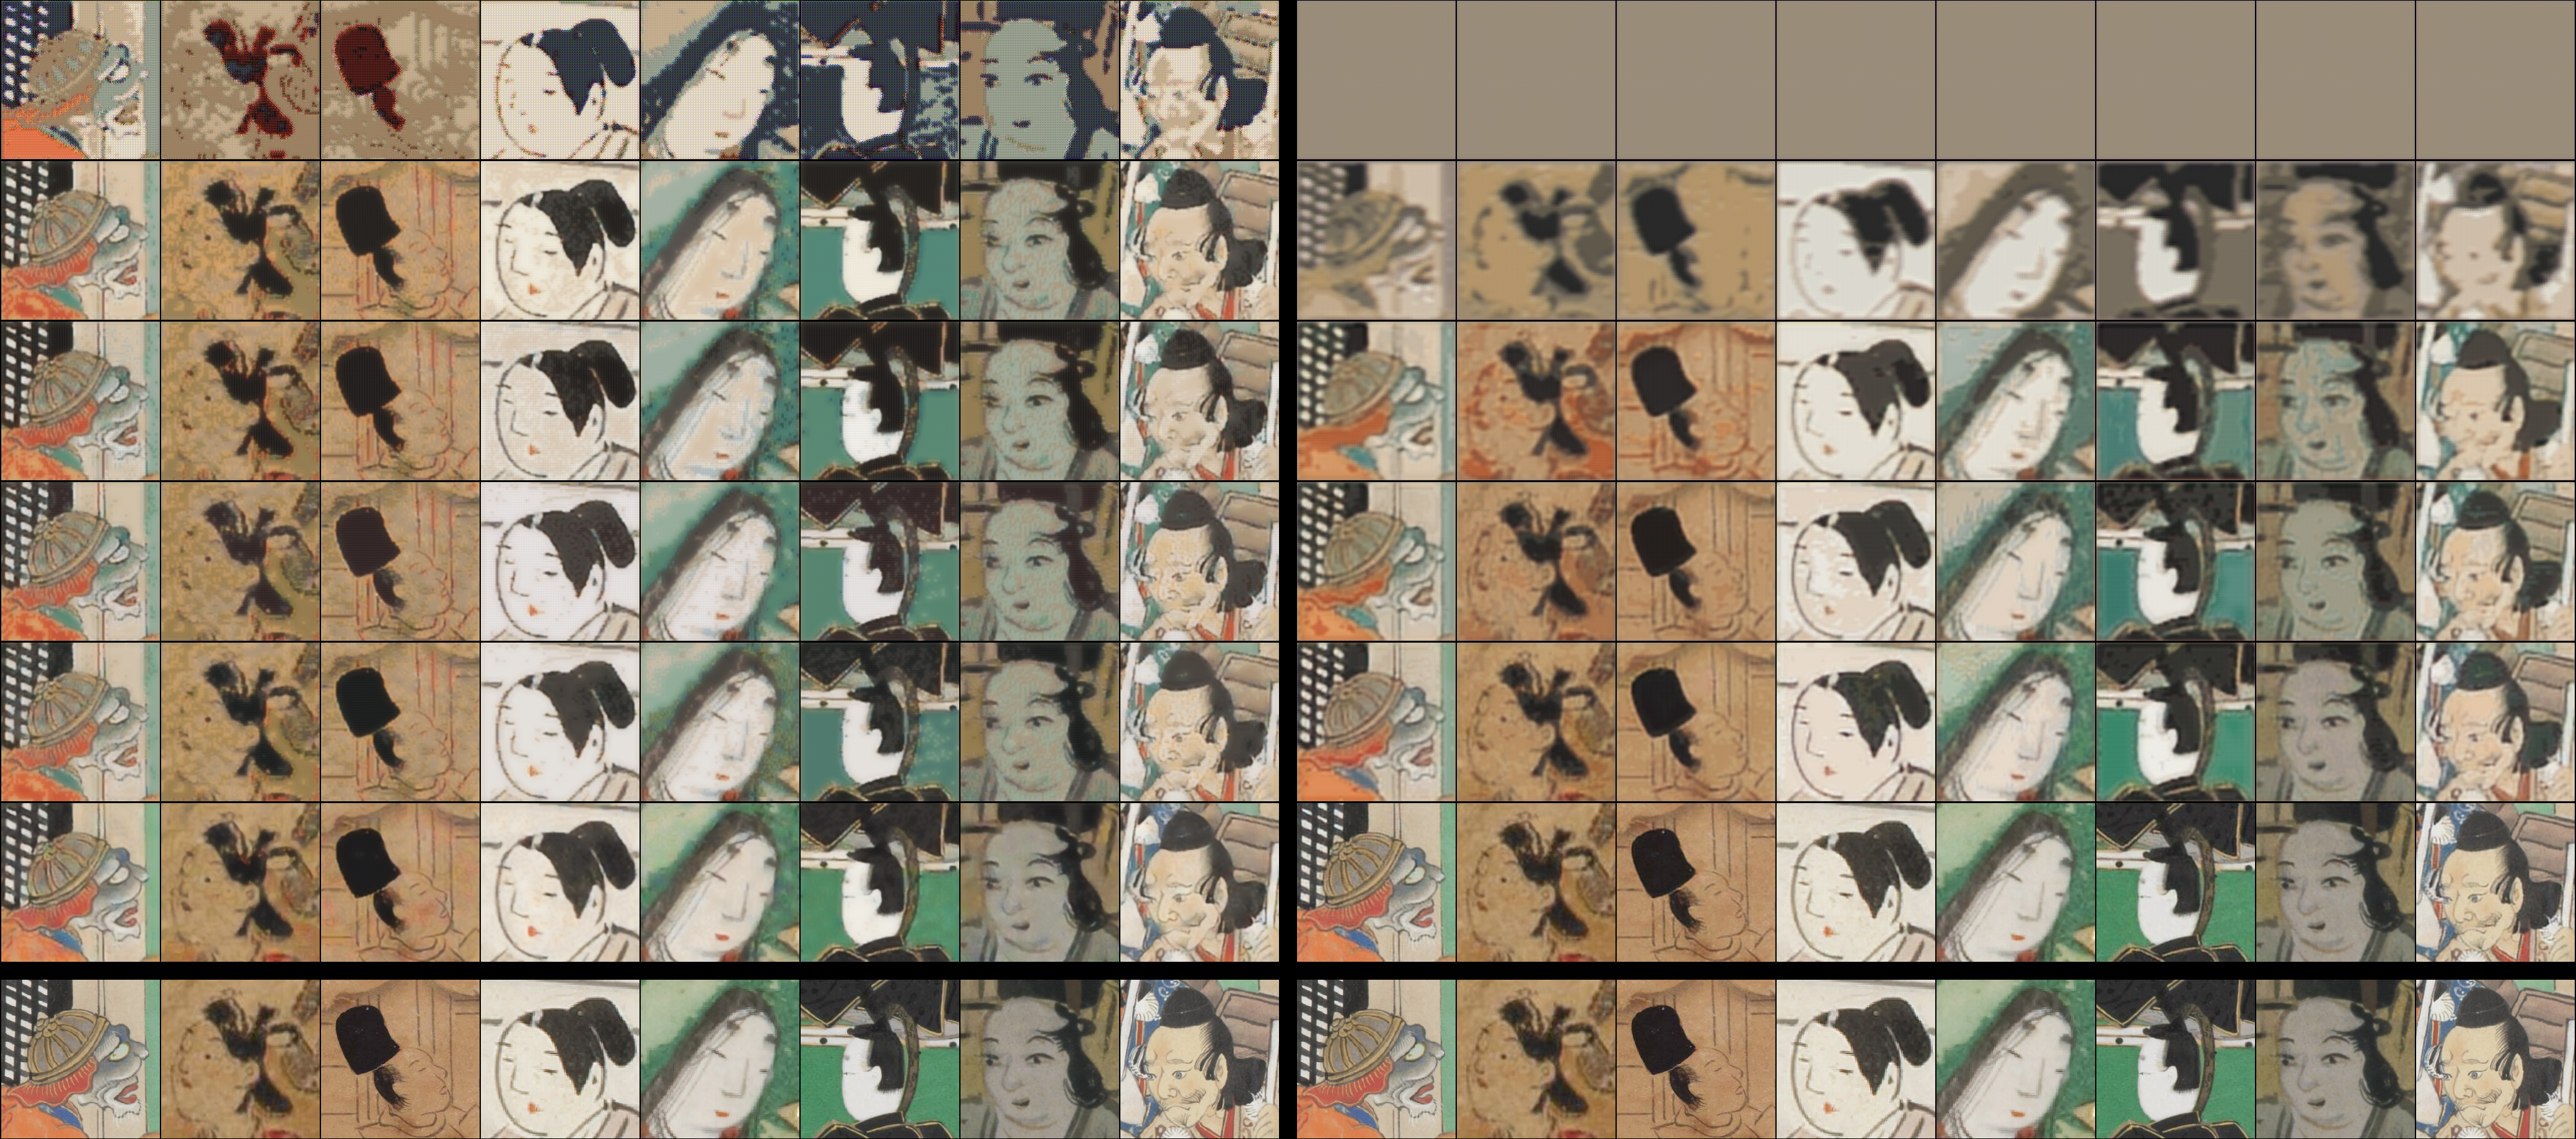
\includegraphics[width=\linewidth]{samples.png}
    \caption{The first six rows of images show samples at 1, 12, 14, 16, 18, and 100 epochs for VQ-VAE (left) and VQ-VAE2 (right). The final row shows the cooresponding images from the testset.}
\end{figure}

As indicated in table...

\section{Conclusion}

The authors of the VQ-VAE paper presented promising results. However, bsaed on our experiments, we conclude that it is not strictly better than VAE on every dataset...

\end{document}